% !TeX encoding = UTF-8

\documentclass{protokol}

\usepackage{tikz}
\usetikzlibrary{calc}
\usetikzlibrary{arrows}

%====== Units =====
\usepackage{siunitx}
\sisetup{inter-unit-product =\ensuremath{\cdot}}
\sisetup{group-digits = integer}
\sisetup{output-decimal-marker = {,}}
\sisetup{exponent-product = \ensuremath{\cdot}}
\sisetup{separate-uncertainty}
\sisetup{tight-spacing = false}
%\sisetup{scientific-notation = true}
%\sisetup{round-mode=places,round-precision=4}
%\sisetup{evaluate-expression}


%====== Grafy =====
\usepackage{pgfplots}
\pgfplotsset{width=0.8\linewidth, compat=1.17}
\def\plotcscale{0.8}
\usepackage{pgfplotstable}
\usepackage[figurename=Obr.]{caption} % figure caption rename
%====== Rovnice align block ======
\usepackage{amsmath}
\setlength{\jot}{10pt} % rozestup mezi řádky

\graphicspath{ {./img/} }

%====== Vyplňte údaje ======
\jmeno{Jakub Charvot}
\kod{240844}
\rocnik{2.}
\obor{MET}
\skupina{MET/4}
\spolupracoval{Radek Kučera}

\merenodne{10.\,11.\,2022}
\odevzdanodne{24.\,11.\,2022}
\nazev{Operační usměrňovače}
\cislo{4} %měřené úlohy

\predmet{Analogové elektronické obvody}
\ustav{Ústav mikroelektroniky}
\skola{FEKT VUT v Brně}

\def\para{x+0}
\def\parb{\para-80}


\begin{document}
	%====== Vygenerování tabulky ======
	\maketitle
	%====== Úvodní texty protokolu ======

	\section{Teoretický úvod}
		\begin{figure}[h!]
    \centering
    
\includegraphics[width=0.8\textwidth]{schema.png}
    \centering
    \caption{Schémata zapojení -- a) AKO s jedním OZ a tranzostorovým převodníkem úrovně, b) generátor pilových kmitů}
    \label{fig:schema}
\end{figure}



\subsection{Funkce jednotlivých zapojení}

    \subsubsection{Astabilní klopný obvod}

    Základním blokem tohoto zapojení je Schmittův klopný obvod s hysterezí, ten v principu umí na výstupu zobrazovat pouze kladné a zápoorné saturační napětí. Nepřeklápí se v obou směrech stejně, ale až po překročení jisté prahové hodnoty napětí, vzniká tak hysterezní smyčka, viz Obr.~\ref{fig:hystereze-png}.

    \begin{figure}[h!]
        \centering
        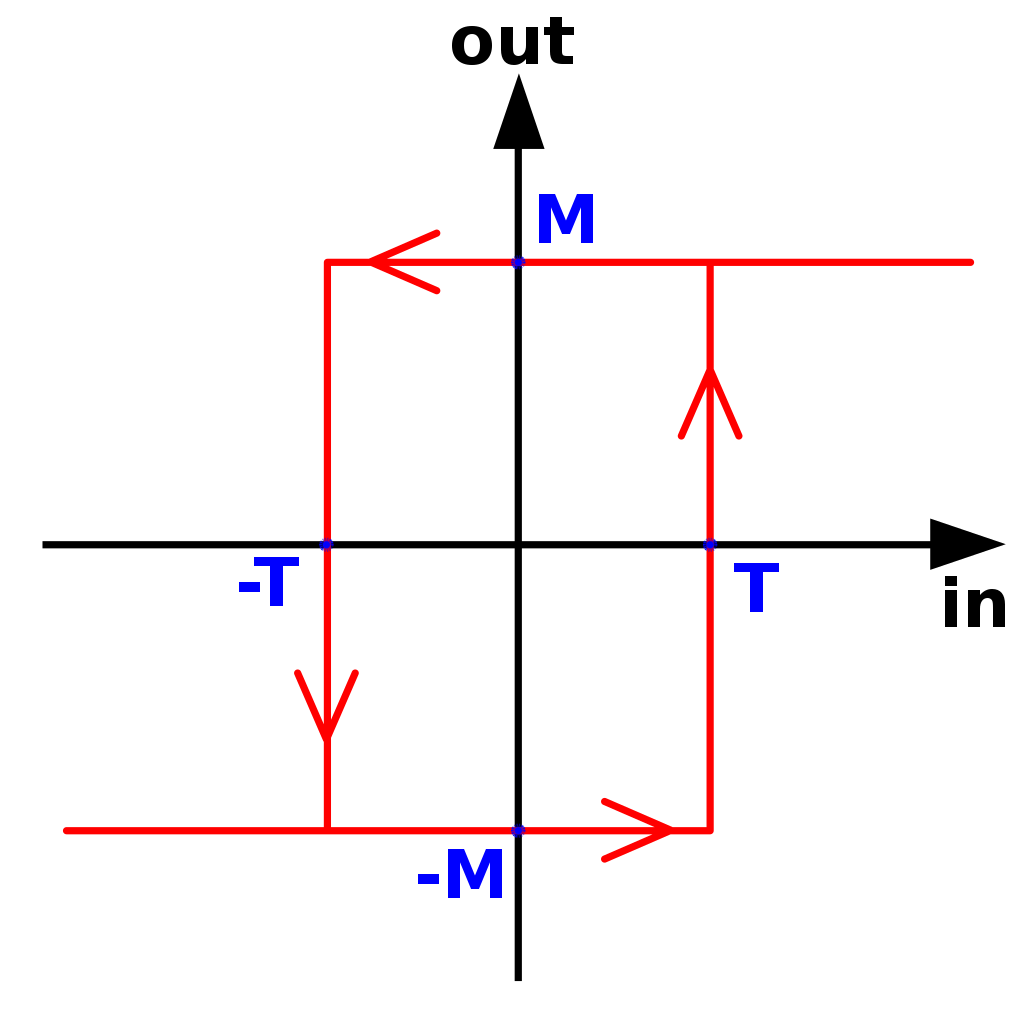
\includegraphics[width=0.5\textwidth]{hystereze.png}
        \caption{Hysterezní smyčka Schmittova klopného obvodu.}
        \label{fig:hystereze-png}
    \end{figure}
    
    Vstup tohoto obvodu je připojen k RC čánku, jehož časová konstanta nám určuje frekvenci překlápění, neboli frekvenci našich vzniklých obdélníkových pulsů, \(F=\frac{0,455}{RC}\).

    \subsubsection{Generátor pilových kmitů}

    Jako základí blok nám opět poslouží komparátor s hysterezí, ke kterému je připojen invertující integrátor, který ze vzniklých obdélníkových kmitů tvoří pilový signál.
    % Operační zesilovač s OZ má za úkol překonat nedostatky, které má zapojení pouze s diodami, které díky svému prahovému napětí nedokáží usměrňovat velmi malá napětí. 
    
    % Zapojení 1a) je jednocestný usměrňovač, kdy je vždy přes jednu diodu uzavřená záporná zpětná vazba a druhá dioda je uzavřená. Na výstupu je pak signál jednocestně usměrněný a invertovaný. 
    
    % Zapojení 1b) pak tento signál zdvojnásobí a sečte s původním vstupním signálem, ve výsledku tedy původní záporné půlvlny zůstanou a kladné po sečtení odpovídají opět záporným. Výsledkem je tedy dvoucestně usměrněný invertovaný signál. 
    % Nevýhodou tohoto zapojení je nutnost použít dva co nejshodnější odpory a k nim jeden, který odpovídá hodnotu přesně polovině, při nedodržení nebudou na výstupu půlvlny stejně velké, toto značně zdražuje zapojení. 

    % Tento problém se snaží řešit zapojení 1c), kdy pro správnou funkci stačí jedna dvojice přesných odporů \( R_2\) a \(R_3\). Záporná zpětná vazba prvního OZ je vždy uzavřena přes druhý OZ, díky diodám je ale cesta zpětné vazby jiná pro kladný a pro záporný signál, takže ve výsledku je na výstupu druhého OZ signál vždy kladný, neboli dvoucestně usměrněný.   
		
	% \newpage
	% \section{Výsledky počítačové simulace}
	% 	% region zapojeniA

\begin{figure}[h!]
    \centering
    \includegraphics[width=0.8\textwidth]{microcap/AKO/1-100kR.png}
    \caption{Zapojení a) OZ 1458 -- Časová závislost napětí v různých bodech obvodu, nejdůležitější je výstup zapojení (červeně) a napětí na kondenzátoru (zeleně), \(R_{p} =\qty{100}{\kilo\ohm}\) . Dále vidíme hysterezní smyčku komparátoru.}
    \label{fig:microcap/AKO/1-100kR.png}
\end{figure}

\begin{figure}[h!]
    \centering
    \includegraphics[width=0.8\textwidth]{microcap/AKO/2-0R.png}
    \caption{Zapojení a) OZ 1458 -- Stejně jako v Obr. \ref{fig:microcap/AKO/1-100kR.png}, jen pro \(R_{p} =\qty{0}{\ohm}\). Zde je již patrné zkosení hran dané mezní rychlostí přeběhu.}
    \label{fig:microcap/AKO/2-0R.png}
\end{figure}

\begin{figure}[h!]
    \centering
    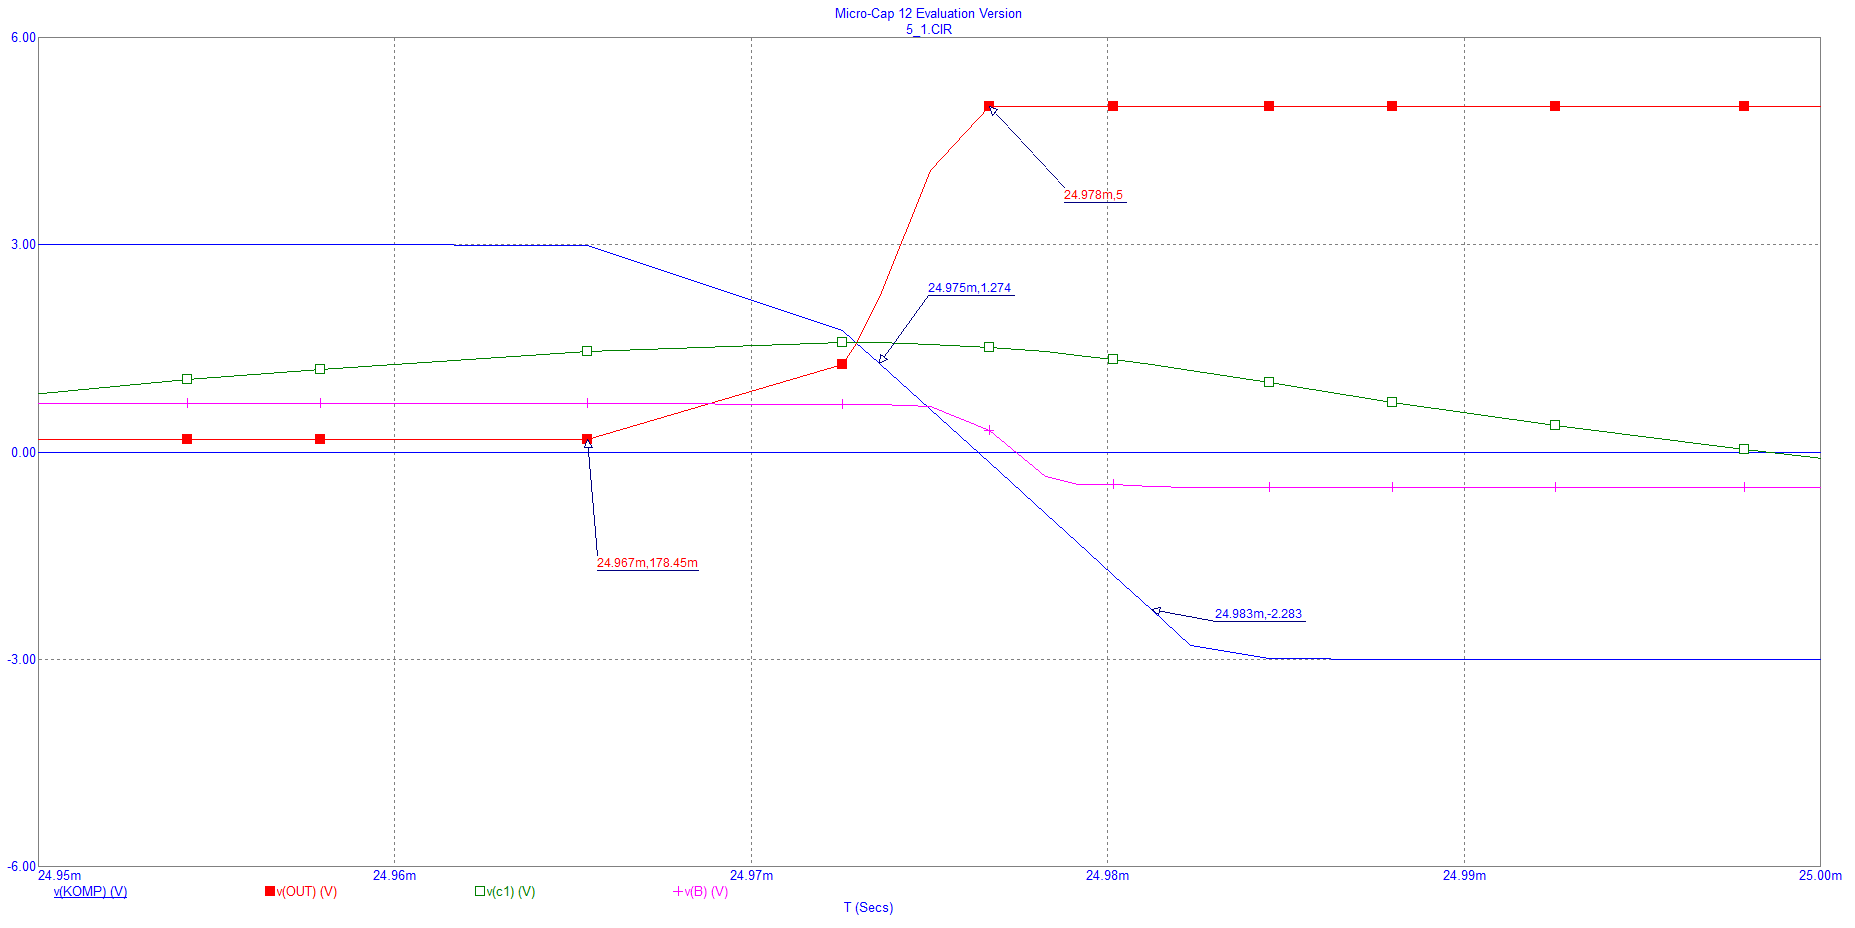
\includegraphics[width=0.8\textwidth]{microcap/AKO/3-strmost0R.png}
    \caption{Zapojení a) OZ 1458 -- Detail náběžné hrany výstupního signálu (červeně) a sestupné hrany signálu na komparátoru (modře).}
    \label{fig:microcap/AKO/3-strmost0R.png}
\end{figure}

\begin{figure}[h!]
    \centering
    \includegraphics[width=0.8\textwidth]{microcap/AKO/4-100k-071.png}
    \caption{Zapojení a) OZ 072 -- Časová závislost napětí v různých bodech obvodu, nejdůležitější je výstup zapojení (červeně) a napětí na kondenzátoru (zeleně), \(R_{p} =\qty{100}{\kilo\ohm}\) . Dále vidíme hysterezní smyčku komparátoru.}
    \label{fig:microcap/AKO/4-100k-071.png}
\end{figure}

\begin{figure}[h!]
    \centering
    \includegraphics[width=0.8\textwidth]{microcap/AKO/5-0R-071.png}
    \caption{Zapojení a) OZ 072 -- Stejně jako v Obr. \ref{fig:microcap/AKO/4-100k-071.png}, jen pro \(R_{p} =\qty{0}{\ohm}\). Zkosení hran je méně výrazné než u OZ 1458, z důvodu lepší hodnoty SR u OZ 072.}
    \label{fig:microcap/AKO/5-0R-071.png}
\end{figure}

\begin{figure}[h!]
    \centering
    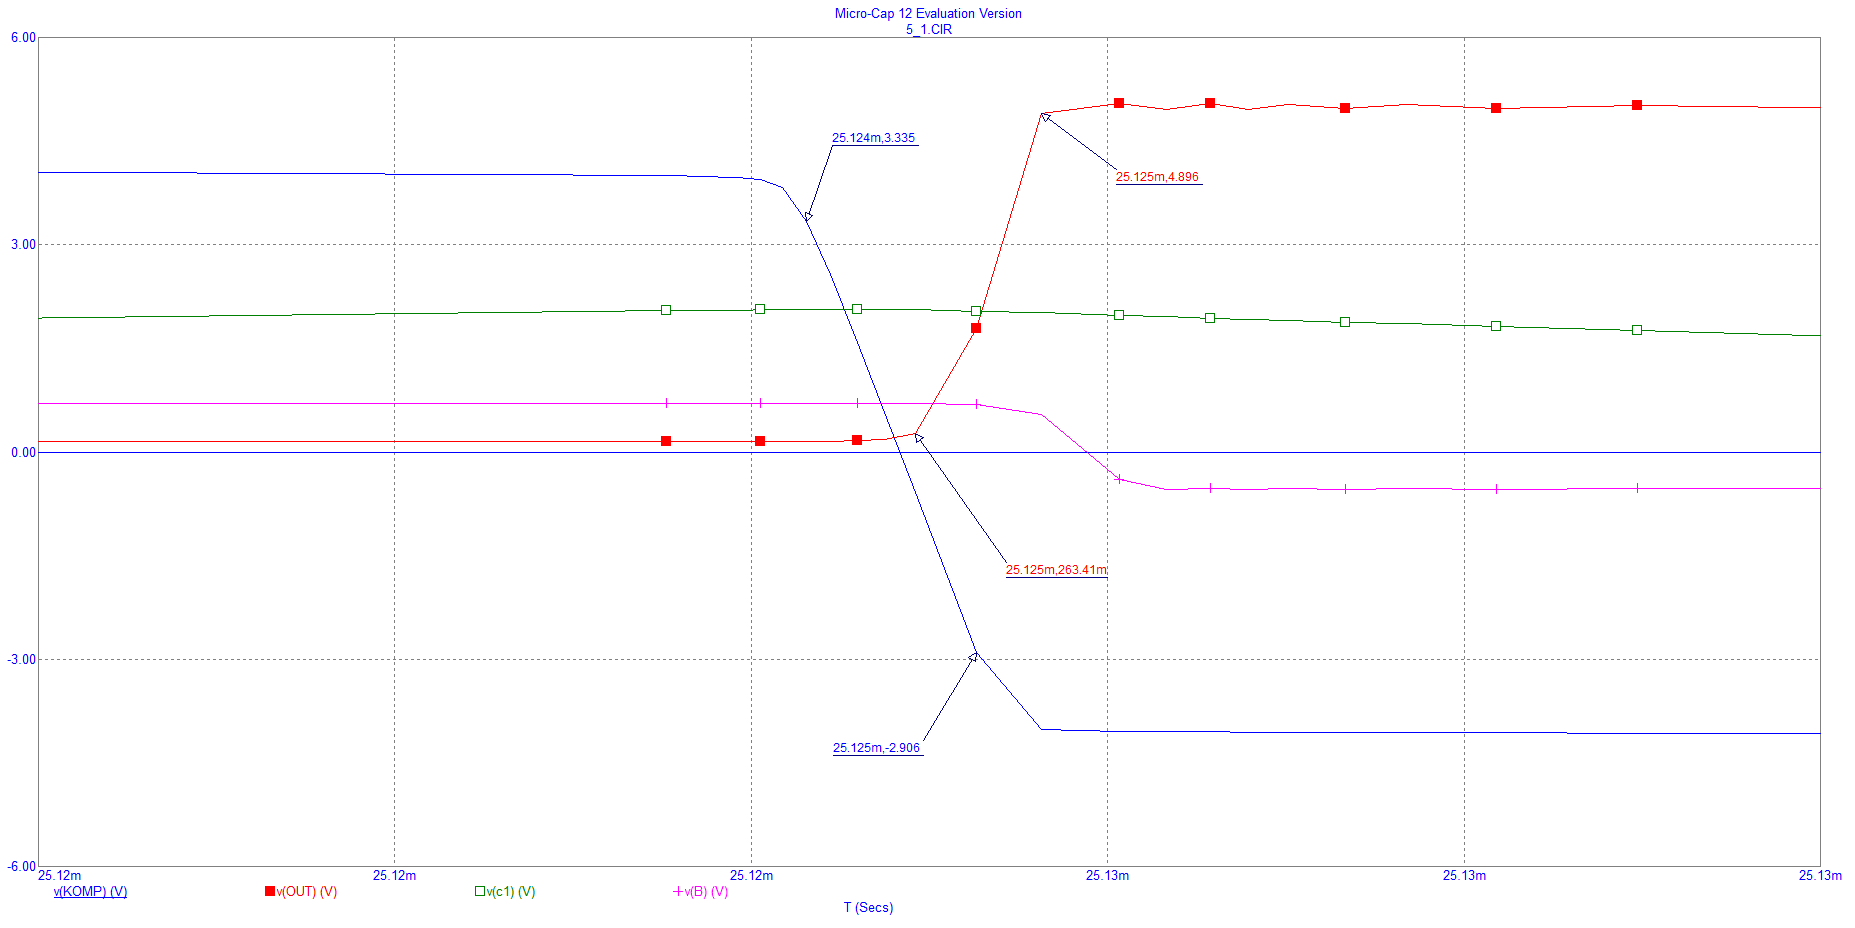
\includegraphics[width=0.8\textwidth]{microcap/AKO/6-strmost0R-071.png}
    \caption{Zapojení a) OZ 072 -- Detail náběžné hrany výstupního signálu (červeně) a sestupné hrany signálu na komparátoru (modře).}
    \label{fig:microcap/AKO/6-strmost0R-071.png}
\end{figure}

% endregion


% region zapojeniB
\begin{figure}[h!]
    \centering
    \includegraphics[width=0.8\textwidth]{microcap/AKO2/1-100kR.png}
    \caption{Zapojení b) OZ 1458 -- Časová závislost napětí na výstupu prvního OZ (obdélník) a druhého OZ (pila), \(R_{p} =\qty{100}{\kilo\ohm}\) . Dále vidíme hysterezní smyčku komparátoru.}
    \label{fig:microcap/AKO2/1-100kR.png}
\end{figure}

\begin{figure}[h!]
    \centering
    \includegraphics[width=0.8\textwidth]{microcap/AKO2/2-0R.png}
    \caption{Zapojení b) OZ 1458 -- Stejně jako v Obr. \ref{fig:microcap/AKO2/1-100kR.png}, jen pro \(R_{p} =\qty{0}{\ohm}\). Opět je zde patrné zkosení hran dané mezní rychlostí přeběhu.}
    \label{fig:microcap/AKO2/2-0R.png}
\end{figure}

\begin{figure}[h!]
    \centering
    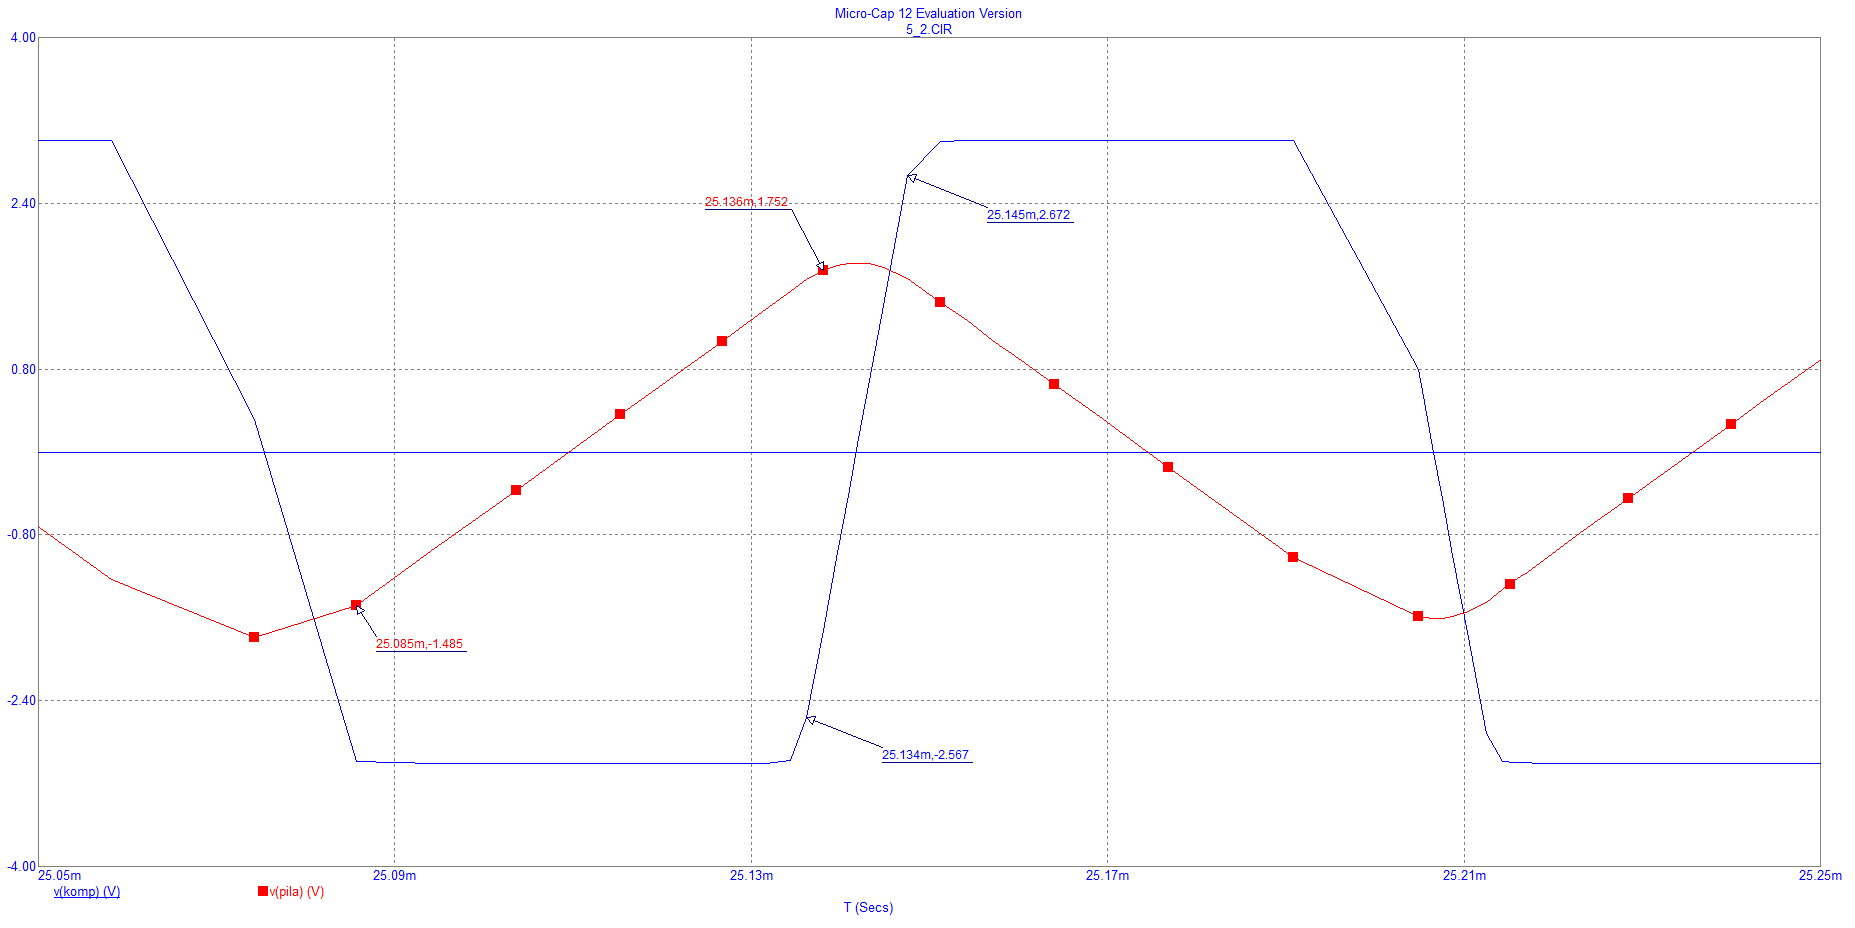
\includegraphics[width=0.8\textwidth]{microcap/AKO2/3-0R-strmost.png}
    \caption{Zapojení b) OZ 1458 -- Detail náběžné hrany signálu na výstupu prvního OZ (modře).}
    \label{fig:microcap/AKO2/3-0R-strmost.png}
\end{figure}

\begin{figure}[h!]
    \centering
    \includegraphics[width=0.8\textwidth]{microcap/AKO2/4-100k-071.png}
    \caption{Zapojení b) OZ 072 -- Časová závislost napětí na výstupu prvního OZ (obdélník) a druhého OZ (pila), \(R_{p} =\qty{100}{\kilo\ohm}\) . Dále vidíme hysterezní smyčku komparátoru.}
    \label{fig:microcap/AKO2/4-100k-071.png}
\end{figure}

\begin{figure}[h!]
    \centering
    \includegraphics[width=0.8\textwidth]{microcap/AKO2/5-0R-071.png}
    \caption{Zapojení b) OZ 072 -- Stejně jako v Obr. \ref{fig:microcap/AKO2/4-100k-071.png}, jen pro \(R_{p} =\qty{0}{\ohm}\). Zkosení hran je minimální.}
    \label{fig:microcap/AKO2/5-0R-071.png}
\end{figure}

\begin{figure}[h!]
    \centering
    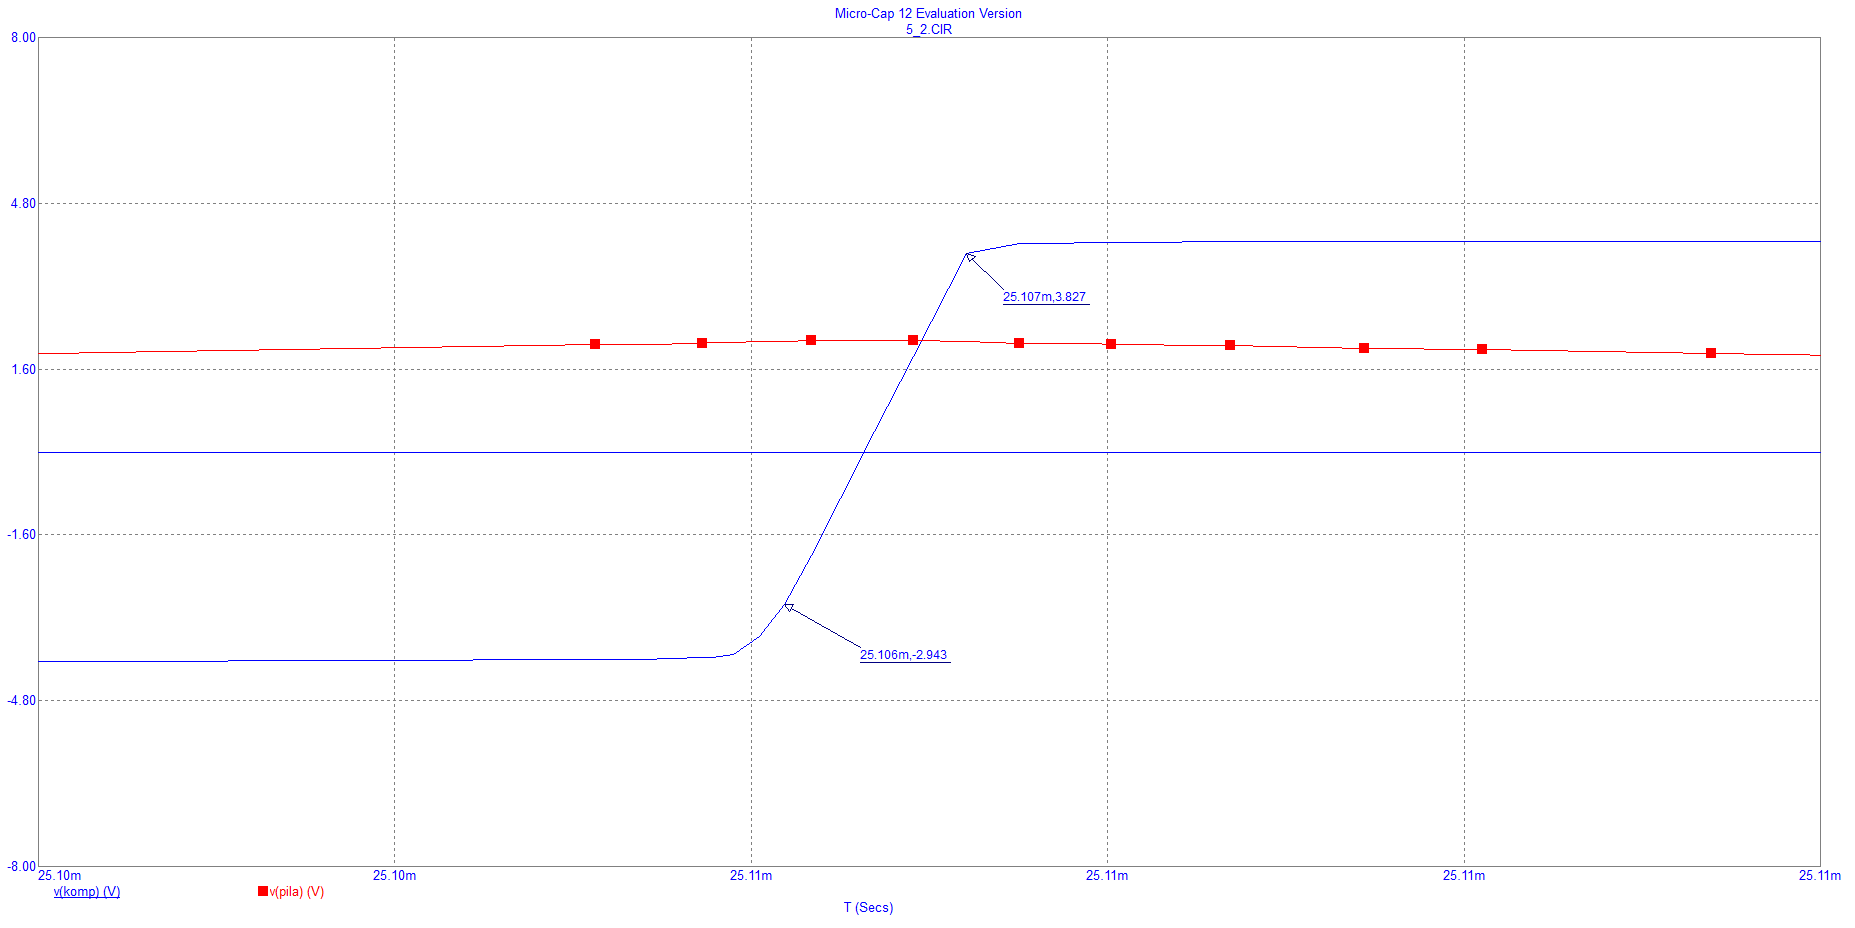
\includegraphics[width=0.8\textwidth]{microcap/AKO2/6-0R-071-strmost.png}
    \caption{Zapojení b) OZ 072 -- Detail náběžné hrany na výstupu prvního OZ.}
    \label{fig:microcap/AKO2/6-0R-071-strmost.png}
\end{figure}

% endregion

	% \newpage
	% \section{Měření v laboratoři}
	% 	% \subsection{Jednocestný usměrňovač}

\begin{figure}[h!]
    \centering
    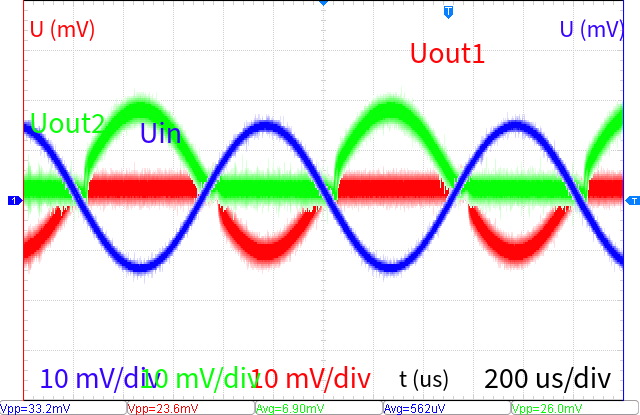
\includegraphics[width=0.8\textwidth]{lab/output3.png}
    \caption{Zapojení a) -- Časová závislost napětí na kondenzátoru (modře) a na výstupu OZ (červeně), \(R_{p} =\qty{100}{\kilo\ohm}\).}
    \label{fig:lab/output3.png}
\end{figure}

\begin{figure}[h!]
    \centering
    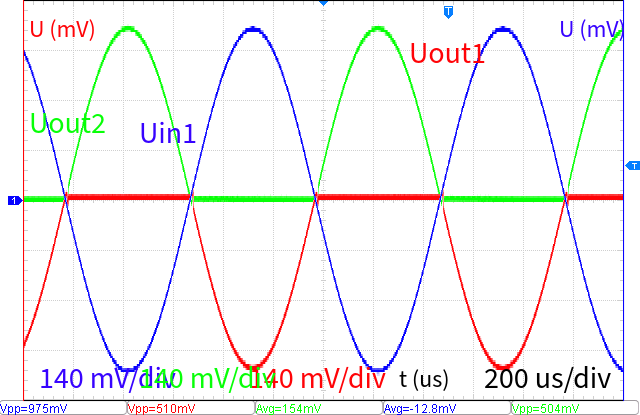
\includegraphics[width=0.8\textwidth]{lab/output1.png}
    \caption{Zapojení a) -- Stejně jako v Obr. \ref{fig:lab/output3.png}, ale pro \(R_{p} =\qty{0}{\ohm}\), je patrné zkreslení dané mezní rychlostí přeběhu.}
    \label{fig:lab/output1.png}
\end{figure}

\begin{figure}[h!]
    \centering
    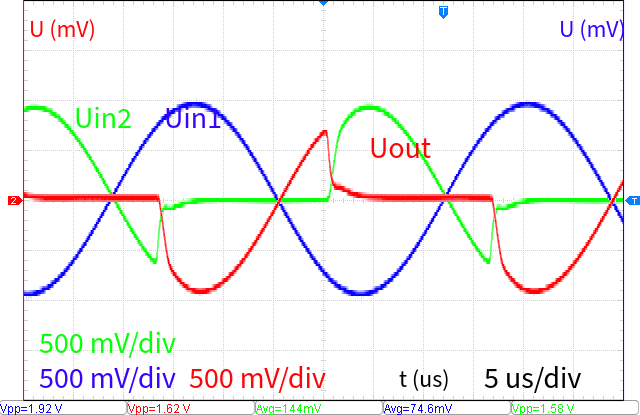
\includegraphics[width=0.8\textwidth]{lab/output6.png}
    \caption{Zapojení b) -- Časová závislost napětí na výstupu prvního OZ (obdélník) a druhého OZ (pila), \(R_{p} =\qty{100}{\kilo\ohm}\).}
    \label{fig:lab/output6.png}
\end{figure}

\begin{figure}[h!]
    \centering
    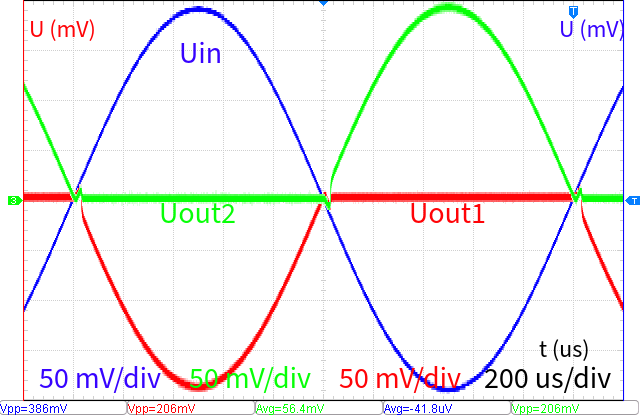
\includegraphics[width=0.8\textwidth]{lab/output4.png}
    \caption{Zapojení b) -- Stejě jako v Obr. \ref{fig:lab/output6.png}, ale pro \(R_{p} =\qty{0}{\ohm}\), opět na této frekvenci vidíme zkosení hran dané nedostatečnou hodnotou SR u tohoto OZ.}
    \label{fig:lab/output4.png}
\end{figure}



\begin{table}[]
    \caption{Porovnání strmostí v simulaci a laboratoři.}
    \centering
    \def\arraystretch{1.4}
    \begin{tabular}{l|l|l|l||l|l|l}
        & \multicolumn{2}{l|}{Zap a) sim} & Zap a) lab & \multicolumn{2}{l|}{Zap b) sim} & Zap b) lab \\ \hline
    typ OZ             & 1458       & 072   & 1458       & 1458       & 072   & 1458       \\ \hline
    \(f_{min} \)  [Hz]      & 100        &   100   & 89         & 108        &    108  & 98         \\ \hline
    \(f_{max} \)  [Hz]      & 8000       &   8000   & 6860       & 7634       &    7634  & 6340       \\ \hline
    S [V/\unit{\micro\second}] & 0,44       & 4,63 & 0,61       & 0,48       & 6,77 & 0,61      
    \end{tabular}
    \label{tab:tabulka_hodnot_brewster}
    \end{table}
		
		
	% \clearpage
	% \section{Závěr}
	% 	U zapojení zesilovače s nesymetrickým napájením jsme nejprve vyhodnocovali stejnosměrný pracovní bod.
	% 	Abychom mohli přenášet kladnou i zápornou periodu signálu, je potřeba tento signál stejnosměrně posunout, aby se ve výsledku i zesílený výstupní signál pohyboval v mezích \qty{0}{\volt} - \(U_{nap} \).
	% 	Tab. \ref{tab:dc-bod} obsahuje porovnání hodnot napětí v jednotlivých uzlech získaných výpočtem, simulací a následně měřením. Tyto hodnoty se téměř neliší a drobná odchylka měřených hodnot je způsobena zejména nedokonalým nastavením napájecího napětí (uzel 1).
	% 	Při změně offsetu např. změnou jednoho z odporů na děliči může dojít k ořezání jedné půlvlny signálu, jak je vidět z obrázků 4 a 13. 

	% 	Dále jsme zkoumali zapojení diferenčního a sumačního zesilovače, odvodili jsme vztah pro výstupní napětí, které by se pro diferenční zesilovač melo rovnat rozdílu obou vstupních. Kromě toho je tedy signál invertovaný. 
	% 	Odečtení signálů jsme pozorovali jak v simulaci (Obr. 9 a 10) tak i v laboratoři (Obr. 14, 15 a 16).

	% 	Funkce sumačního zesilovače je obdobná, odvodili jsme, že na výstupu by měl být invertovaný součet obou vstupních signálů. Simulace součtu signálů se nachází na obrázku 7. V laboratoři jsme zapojení testovali pro dva signály s odlišnou amplitudou i frekvencí (Obr. 17) a také pro součet signálu s nulovým signálem, kdy na výstupu je invertovaná verze prvního vstupního signálu (Obr. 18).

	% 	Všechny průběhy nám vyšly dle očekávání a měření v laboratoři odpovídá předešlým simulacím.
\end{document}